\chapter{Projekt systemu}
W~tym rozdziale zdecyduję, jaką ścieżką pójdę, aby stworzyć oprogramowanie realizujące cele opisane w~punkcie~\ref{lib-requirements}.
Ta decyzja będzie poprzedzona zebraniem wymagań i~prototypowaniem.
Po niej nastąpi szczegółowe projektowanie i~w~końcu implementacja mojego rozwiązania.

%\section{Wybór metodyki}
%Mógłbym tutaj przedstawić po co w~ogóle są metodyki wytwarzania oprogramowania, przeanalizować najpopularniejsze i~jakąś wybrać, pewnie dostosowując jeszcze do swoich potrzeb.
%Np. na początku podział na zwinne i nie. Mi oczywiście pasują zwinne, bo nie jestem gigantycznym projektem. Poza tym zwinne są lepsze i RUP to tylko nieudana teoria.
%Potem powiedzieć, co to Scrum i że nie potrzebuje, bo nie mam zespołu.
%Potem Extreme Programming przedstawić, i powiedzieć, że ma Spajki, a to jest coś, co mi się przyda.
%Jakieś linki do tego:
%http://servicevirtualization.com/profiles/blogs/when-agile-is-not-enough
%https://www.scrum.org/resources/what-is-scrum/

%\section{Metodyka wytwarzania(TODO)}
%Zdecydowałem, że tworząc mój projekt będę postępował zgodnie Zabierając się za projekt informatyczny dobrze sobie obrać jakąś metodykę (źródło).
%Ja zdecydowałem się na pewną wersję Xtreme programming.
%Jeśli będę robił jakieś większe schematy to będzie to zapożyczenie z~cięższych metodyk, niejako potrzebne dla naukowego aspektu pracy.

\section{Specyfikacja wymagań systemowych (SWS)}
Z~celów tej pracy zawartych w~punkcie~\ref{lib-requirements} stworzyłem standardową listę konkretnych wymagań dla zespołu inżynierów, czyli mnie samego.
Organizując niniejszą sekcję wzorowałem się na specyfikacji wymagań systemowych opisanej w~prezentacji ,,Inżynieria Wymagań'' Jarosława Kuchty, z~przedmiotu ,,Dokumentacja i~Jakość Oprogramowania''\cite{kuchta}.


\subsection{Wstęp i~opis informacyjny}
Jako rozbudowana sekcja wstępu SWS oraz ,,szczegółowy opis problemów do rozwiązania'' służyły poprzednie rozdziały niniejszej pracy.


\subsubsection{Diagram przepływu najwyższego poziomu}
Diagram~\ref{fig:project-overview} przedstawia ogólne działanie systemu w~trakcie wywoływania zdalnej metody. Jest to główna funkcja mojego projektu. Funkcja drugorzędna -- tłumaczenie danych, również została ujęta.

Widoczny na schemacie klient jest jednym z~wielu, które mogą być stworzone przez kod korzystający z~mojej biblioteki.
Obiekt każdego klienta spełnia jakiś zadany interfejs. Robi to przez opakowywanie parametrów, zaadresowanie ich, wysłanie do obiektu faktycznie wykonującego kod i~odebranie wyniku.
Interfejs klienta i obiektu zdalnego są zgodne, chodź napisane w~różnych językach na różne platformy. Aby zminimalizować nakład pracy programisty, najlepiej byłoby, gdyby interfejs po stronie klienta (.NET) był generowany z~wersji serwerowej (Java, Android).
Tak samo jak w~przypadku interfejsów wygląda sprawa klas przekazywanych do metod jako parametry -- także muszą być zgodne, najlepiej automatycznie tłumaczone.
Typy przetłumaczone na schemacie oznaczone są apostrofem.
Kod kliencki nie musi zawierać tłumaczenia implementacji zdalnych interfejsów.
Współdzielone definicje klas danych i~interfejsów są niezbędne, aby uzyskać polimorfizm metod zdalnych.

Serwer jest tworzony przez kod kliencki i~nasłuchuje na żądania na zadanym interfejsie sieciowym. Może to być dowolna technologia pozwalająca na dwustronne wysyłanie wiadomości, np.\ TCP, HTTP, SSL/TLS, czy też strumienie w~pamięci (rozwiązanie lokalne).
Na schemacie serwer posiada tylko jeden obiekt zdalny klasy \texttt{Implementacja A}, ale faktycznie może posiadać ich wiele.

\begin{figure}
	\centering
		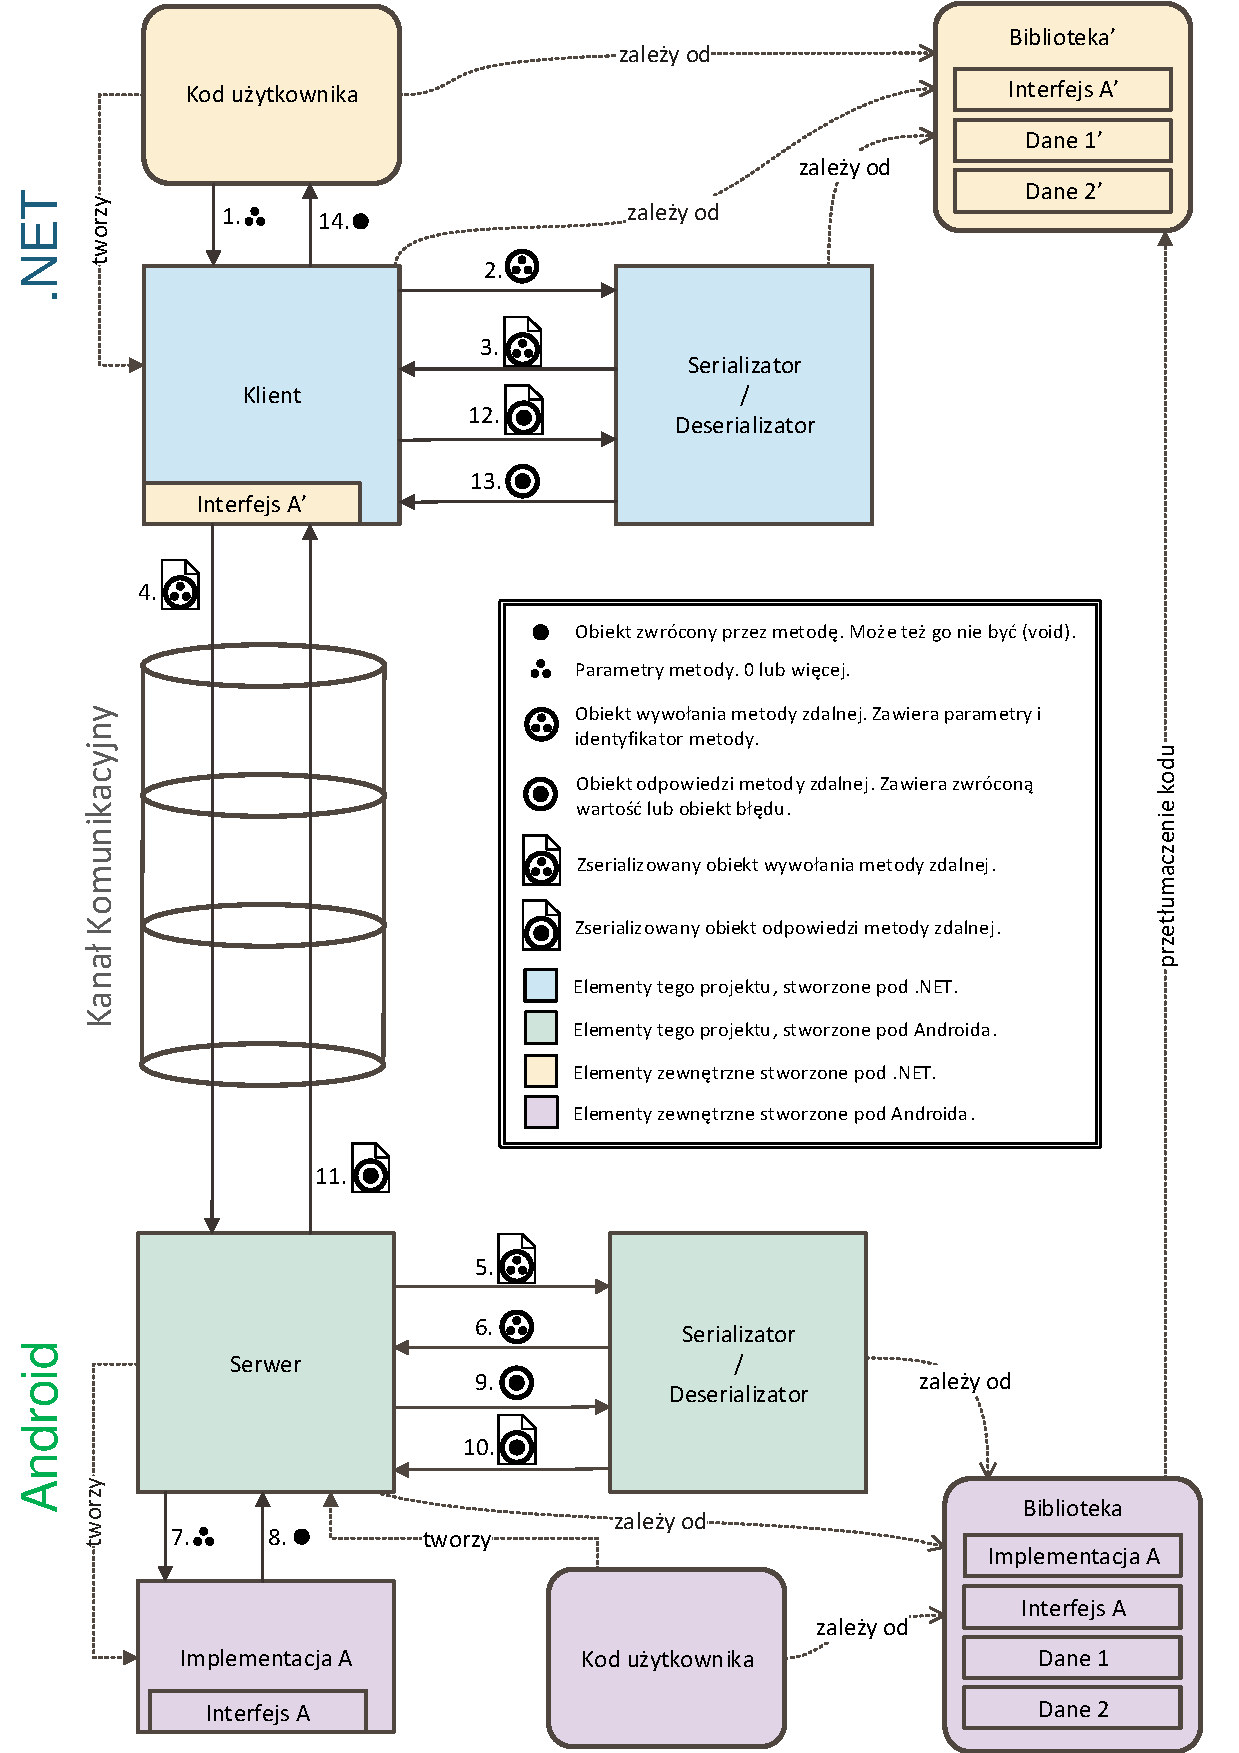
\includegraphics[scale=0.8]{img/schematy/schemat-dzialania-magisterki.pdf}
	\caption{Ogólny schemat projektu.}
	\label{fig:project-overview}
\end{figure}


\subsubsection{Reprezentacja zawartości informacyjnej}
Nie można właściwie mówić o~zawartości informacyjnej systemu, ponieważ takiej nie będzie.
Przez mój system dane będą jedynie przepływać.


\subsubsection{Opis interfejsów systemowych}
\begin{itemize}
	\item Jako, że to, co tworzę będzie kolekcją bibliotek Javy i~C\# będą one mogły być ładowane, a~ich klasy wykorzystywane przez zewnętrzne aplikacje.
	\item Niezależne narzędzie do generacji kodu będzie opatrzone w~interfejs linii poleceń.
\end{itemize}


\subsection{Wymagania funkcjonalne}
%opis tekstowy
%ograniczenia
%wymagania wydajnościowe
%zastrzeżenia projektowe
%diagramy pomocnicze
% WYMAGANIA POMIJANE:
% reliable sessions (w sumie też by mi się przydał jakiś mechanizm, który umożliwi komunikację w niestabilnym środowisku Internetu)
% \url{http://blogs.msdn.com/b/shycohen/archive/2006/02/20/535717.aspx} \\

\subsubsection{Ogólne}

\begin{description}
\itemtitle{Serializacja danych z zachowaniem informacji o typach}
Zserializowane reprezentacje obiektów muszą zawierać informacje o~typach wtedy, kiedy nie wynika ona jednoznacznie z~kontekstu.
Np.\ przy zwracaniu ze zdalnej metody obiektu klasy dziedziczącej po tym, zdeklarowanym w~interfejsie tejże metody.
To wymaganie dotyczy zarówno strony klienta jak i~serwera.
Deserializacja powinna być komplementarna i~ze stworzonych reprezentacji odtwarzać obiekty o~odpowiednich typach i~z~poprawnymi danymi.
Taka metoda serializacji i~deserializacji jest warunkiem działania polimorficznych metod.

\itemtitle{Tłumaczenie kodu}
Zrealizowane jako niezależne narzędzie.
Tłumaczenie kodu zmniejszyłoby nakład pracy programisty, który bez tego musiałby sam stworzyć odpowiadające klasy danych w~obu językach.
Klasy i~pola nie znajdujące odpowiednika są pomijane w~trakcie tłumaczenia.
Tłumaczenie powinno się odbywać z~Javy do C\#, ponieważ w~Javie będzie więcej kodu (kod implementacji zdalnych metod).
%Jeśli w danej klasie są inne klasy z zewnętrznej biblioteki, to trzeba też przetłumaczyć te. Trzeba dostarczyć kod wszystkich.
%Jeśli jedno ogniwo jest nieprzetłumaczalne to można pominąć pole z ostrzeżeniem.
\end{description}

\subsubsection{Serwer}

\begin{description}

\itemtitle{Komunikacja z~klientem}
Serwer powinien nasłuchiwać na żądania od klientów na zadanym dwustronnym kanale komunikacyjnym.
Konkretny typ kanału (TCP, SSL, HTTP, itp.) nie jest ważny.
Może przyjmować wywołania metod i~przekierowywać je do obiektów zdalnych (względem klienta).
Przekazuje do klientów zwracane wartości.

\itemtitle{Wystawianie metod publicznych zadanych obiektów ,,na zewnątrz''}
Kod serwera ma przyjmować dowolny obiekt i~umożliwiać zdalnym klientom wywoływanie jego publicznych metod.
Parametry tych metod muszą być przetłumaczalne na kod klienta.

% Można się też zastanowić nad singletonami.
\itemtitle{Tworzenie zdalnych obiektów na życzenie klienta}
Po otrzymaniu specjalnego żądania kod serwera powinien stworzyć obiekt implementujący zadany interfejs i~zwrócić jego identyfikator. Klient będzie mógł wywoływać zdalnie metody na stworzonym obiekcie.

\itemtitle{Niszczenie zdalnych obiektów na życzenie klienta}
Specjalne żądanie zawierające identyfikator obiektu powinno powodować jego zwolnienie i~uniemożliwienie z~nim dalszej komunikacji.

\itemtitle{Polimorfizm parametrów metod zdalnych}
Metody zdalne muszą obsługiwać parametry wszystkich typów zgodnych ze spodziewanym. Dla przykładu, metoda przyjmuje parametr typu A, więc powinna przyjąć też parametry wszystkich typów dziedziczących po A.

\itemtitle{Przeciążanie metod zdalnych}
Metody zdalne mogą być przeciążane, tj.\ dwie metody mogą mieć tę samą nazwę, ale inny zestaw parametrów.

\itemtitle{Komunikacja z systemem Android}
Obiekty zdalne muszą mieć możliwość wywoływania metod z~API Androida.

\end{description}

\subsubsection{Klient}

\begin{description}

\itemtitle{Tworzenie obiektów klienckich}
Biblioteka po stronie .NET musi być w~stanie dynamicznie stworzyć obiekt klienta dla obiektu zdalnego.
Każdy klient spełnia jakiś zadany interfejs.

\itemtitle{Nawiązywanie sesji z~serwerem}
Obiekt klienta nawiązuje kontakt z~serwerem poprzez dowolny dwustronny kanał komunikacyjny (na którym serwer nasłuchuje).
Następnie żąda od serwera stworzenia dla siebie zdalnego obiektu.
Wszystkie metody z~interfejsu zdalnego wywoływane na kliencie są przekazywane do jednego obiektu zdalnego.
Zwolnienie obiektu klienta powoduje zwolnienie obiektu zdalnego.

\itemtitle{Konsumowanie polimorficznych metod zdalnych}
Klient wykonuje metody implementowanego przez siebie interfejsu przez delegację (i~wysłanie) ich do obiektu zdalnego.
Wysłanie poprzedzane jest serializacją, podczas której muszą zostać zachowane informacje o~typach parametrów oraz ich ewentualnych obiektach składowych.

\end{description}


\subsection{Wymagania niefunkcjonalne}

\begin{description}

\itemtitle{Serwer na Androidzie}
Kod serwera musi działać na platformie Android.

\itemtitle{Klient w~.NET pod Windows}
Kod klienta musi działać na platformie .NET\@.

\itemtitle{Wydajność serwera}
Nie musi być duża, jako, że nie jest priorytetem projektu. Wystarczy jednoczesna obsługa pięciu (5) klientów.

\itemtitle{Rozszerzalność metod zdalnych bez ingerencji w oryginalny kod}
Funkcjonalność metod zdalnych powinna być rozszerzalna bez ingerencji w~ich kod dzięki mechanizmom programowania obiektowego.
Przykładem jest możliwość przyjmowania przez metodę zdalną obiektu klasy dziedziczącej po spodziewanym typie parametru, bez potrzeby jakiejkolwiek ingerencji w~kod metody, aby mogła rozumieć nową klasę.
Jednak definicja nowej klasy musi być dostępna zarówno dla klienta, jak i~serwera.

\itemtitle{Łatwość użytkowania}
Budowanie i~korzystanie z~bibliotek, które powstaną w~trakcie realizacji tego projektu, powinno być proste i~intuicyjne.

\end{description}



\section{Prototypy}
Aby dokładnie zaplanować strukturę i~działanie mojego oprogramowania muszę zebrać więcej informacji.
Także pomysły, jakie mam na rozwiązanie problemów tej pracy, wymagają weryfikacji.
W~tej sytuacji dobrze przygotować kilka małych prototypów lub jak to określają wytyczne programowania ekstremalnego\footnote{Z~ang. \emph{eXtreme Programming}, w~skrócie XP.} -- \emph{,,spike solutions''}, czyli rozwiązania -- gwoździe lub kolce\cite{spike}. Nazywają się tak, ponieważ przeszywają/przechodzą przez wszystkie warstwy projektu.

Poniżej znajdują się opisy przygotowanych przez mnie ,,\emph{spike'ów}''.

\subsection{Wspólny format informacji o typach (TODO)}
Zarówno część na Androidzie jak i~.NET musi tak samo oznaczać typy obiektów w~zserializowanych obiektach.
Jest to podstawa do uzyskania polimorficznych zdalnych metod.
Chcę to zrobić przez dobranie serializatorów po obu stronach i~odpowiednią ich konfigurację. Ewentualnie będę ingerował w~ich kod.
Myślę o~Jackson po stronie Androida i~DataContractJsonSerializer lub JSON.NET po stronie .NET\@.

Zrobię zmianę źródeł JSON.NET, żeby to \$type było konfigurowalne. Tworzę swój SerializationBinder i wszystko wygląda tak, jak w Jacksonie.
%http://stackoverflow.com/questions/9490345/json-net-change-type-field-to-another-name
%http://james.newtonking.com/archive/2011/11/19/json-net-4-0-release-4-bug-fixes
%http://blog.maskalik.com/asp-net/json-net-implement-custom-serialization/

%\subsubsection{Wyniki}
%I~co, ma to sens? Udało się?


\subsection{Polimorficzne metody zdalne(TODO)}
Trzeba ustawić zgodne polimorficzne serializatory zarówno dla klienta jak i~serwera i~wywołać jakąś z~metod, którymi testowałem polimorfizm w~rozdziale~\ref{similar-technologies}.
Zastosuję jsonrpc4j (jeśli Jackson w~pierwszym prototypie się spisał) na Androidzie i~JSON-RPC.NET po stronie .NET\@.
Opieranie się o~standard Json-Rpc daje ,,gratis'' identyfikatory połączeń i~wysyłanie błędów.

\subsection{Tworzenie zdalnych obiektów na żądanie klienta(TODO)}
Klient musi mieć specjalną metodę, którą będzie wywoływał stworzenie zdalnego obiektu, któremu dalej będzie wysyłał wywołania.
Można to zrealizować przy pomocy mechanizmu rozszerzeń (\emph{Extensions}) standardu JSON-RPC 2.0.
%https://jsonrpcx.org/Main/HomePage
%http://grokbase.com/t/gg/json-rpc/138ce80p54/what-are-rpc-extensions



\section{Szczegółowy projekt (TODO)}
Tutaj decyzja, co do ostatecznego kształtu rozwiązania, szczegółowy plan struktury i~działania.

\subsection{Wybrana ścieżka}
Jakie prototypy wybieram do dalszego rozwinięcia?
Dlaczego?


%\subsection{Przypadki użycia}
%Jakie są? Do czego można użyć tego systemu? Jak to jest z tym dynamicznym tworzeniem web serviceów z hierarchii klas?


\subsection{Struktura projektu}
Diagramy warstwowe, komponentowe, klas.

%Napisać, co jest potrzebne dla remotingu: jakaś tożsamość, adres obiektu, oznaczenia metod, argumentów. Ogólnie to jest dość proste. (jak w~JSON-RPC, tylko z polimorficznymi typami)


\subsection{Schemat działania projektu}
Schematy działania, to z liniami życia, diagramami aktywności itp.


\subsection{Plan testów}
Jakie testy akceptacyjne? Jak sprawdzę, że działa? Na jakiej konfiguracji sprzętowej będę musiał to robić?

Tworzenie grafu w~typów w~xmlu? Są obiekty, które mogą mieć dzieci (tablice, listy). Próbuję wygenerować C\# dla porównania. Zapisuję grafy, które nie działają (w trakcie automatycznych testów). Zrobić wizualizator grafów?


%Budowa powinna pozwolić na łatwe podłączenie warstwy bezpieczeństwa (bezpiecznego kanału)
%
%Call:
%- id obiektu (0 dla tworzenia nowego, wtedy argumentem jest tym)
%- id metody
%- parametry
%
%Response:
%- czy sie udalo
%- obiekt zwrotny, opis błędu przy wywołaniu zdalnej metody lub stacktrace z exceptiona, który wystąpił w metodzie
%
%Id metody:
%składa się z nazwy i aliasów jej parametrów.
%
%Alias:
%typy prymitywne - int, string, itp.
%datacontract - sraka:\#ptaka.daka
%lista - List
%tablica - [int, [[int, [sraka:\#ptaka.daka, itp.
%
%Tłumaczenie aliasów:
%C\# tłumaczy klasy na aliasy, jak przetłumaczy dla jednej metody to dodaje to do słownika, żeby potem robić to od razu.
%Java tłumaczy aliasy na nazwy klas (potem loaderem). Wiąże w słowniku id metody z obiektem metody. Może być metoda przyjmująca jakiś konkretny List, np. ArrayList, ale nie może mieć overloada przyjmującego inny List.
%Kiedy czyścić te słowniki?
%
%Loader:
%Loaduje aliasy DataContractów, klasy javowe, klasy serwisów(?). Czyta sobie jary, szuka adnotacji
%
%Typy danych i serwisy w javie są oznaczone namespaceami, odpowiadających im rzeczy z C\# (DataContracty i interfejsy)
%
%Oddzielić abstrakcje od sposobu transportu. Wyróżnic transport streamowany (serializator dostaje strumień i na niego wali output, możemy tłumaczyć i wysyłać na raz) i nie (trzeba stworzyć całą wiadomość, wtedy wysłać).
%
%Zrobić timeouty na łączenie do serwisu i na operacje. Poczytać więcej o TCP, zobaczyć, czy dobrze można nim sprawdzać, czy trzeba używać PINGa.
%
%Serializujemy wszystkie publiczne pola/ propertiesy albo metody z get / set (to w Javie). Używać jakiś dostępnych już atrybutów do ręcznej konfiguracji wyboru serializowanych elementów.



%Dobrze korzystać z~istniejących standardów. Wprowadzenie nowego standardu nie jest dobrą rzeczą, chyba, że ma się ogromną rzeszę zwolenników lub naprawdę poważne przesłanki (powody). Kto wie, może takie mam. Ale na ogół lepiej kombinować istniejące rozwiązania tak, żeby zewnętrzne komponenty miały szansę na współpracę z nimi.
%
%Pomysły do SPIKEów będę wybierał na bazie doświadczenia (i~przesłanek opisanych poniżej w~\ref{approach-selection}).
%Będę starał się wykorzystać jakieś badane wcześniej technologie. Bo lepiej używać gotowych, dojrzałych komponentów tam, gdzie można. Po co wymyślać koło od nowa?
%Spike'i będę tworzył w~kolejności od tego, który według mnie ma największe prawdopodobieństwo na bycie prototypem ostatecznego rozwiązania.
%Może się nawet udać za pierwszym razem, ale na wszelki wypadek powinienem zrobić kilka. Bo a~nóż się okaże, że mój drugi albo trzeci wybór będzie się zachowywał lepiej.
%
%\subsection{Selekcja podejść}
%\label{approach-selection}
%Jakie podejścia, techniki odrzucam, na jakich się skupię, dlaczego?
%
%\subsubsection{Dlaczego nie chcę pisać serializacji}
%To dużo roboty i~zostało zrobione wiele razy. Jak już to bym wziął istniejący projekt, zrobił fork i~dodał wpisywanie i~odczytywanie informacji o~typach. Może nawet potem bym swoje zmiany dodał do oryginalnego projektu?
%
%\subsubsection{Dlaczego nie Schemy i referencje we wiadomościach}
%Chyba nie zależy mi na referencjach, jak linki do schem w SOAPie. System ma być prosty, wiadomości spójne i pełne. Odniesienia powodują dużo skomplikowanie, które jest zbędne - całe dane powinny być zawarte w wiadomości. A no i ja się nie bawię w schemy, nie przesyłam opisu danych (te są w klientcie i serwerze), przesyłam tylko surowe dane.
%
%\subsubsection{Dlaczego nie REST}
%Nie zależy mi konkretnie na łączności przez internet, a~to jest podstawowym założeniem RESTa.
%Chcę wspierać wiele warst transportowych, nie tylko HTTP. Poza tym parsowanie adresów jest bardziej problematyczne niż proste pobieranie nazw metod.
%
%Będę robił raczej RPC z~JSONem, nie będę udawał RESTa.
%WADL nie jest w~ogólności zbyt potrzebny, bo REST może bez niego żyć.
%
%\subsubsection{Dlaczego nie SOAP}
%Nie uważam, że skomplikowanie SOAPa jest odpowiednie do RPC\@. Wystarczy zobaczyć, jak ciężko jest skomunikowac sie z serwisem w WCF przy pomocy kSOAP - ktos wlozyl w to duzo roboty, a i tak w minimalnie bardziej zaawansowanych (tablice?) przypadkach ciezko sprawic, zeby dzialalo. Tylko duze implementacje na duze platformy daja rade.
%
%W generację WSDLa nie chcę się babrać - skomplikowane.
%
%Namespace'y są ważną rzeczą w SOAPie. Ja twierdzę, że nie są potrzebne w tak rozbudowanej formie. Może być jedno standardowe nazewnictwo z kropkami. Zakładam taki jakby jeden globalny namespace na oba runtime'y (klient i serwer). Fakt, że nawet jedna strona może mieć kilka przestrzeni nazw (parę class loaderów albo assembly cache'y) ale nie chcę tego robić z uwagi n utrudnienia w integracji (tu można napisać jakby to mogło wyglądać, ale nie trzeba, mogę po prostu to olać).

%\section{Inne SPIKE'i}
%
%\textbf{Serializacja JSONa (raczej samej serializacji nie chcę robić):}
%Przejrzeć specyfikację, zobaczyć, z czym musieli sobie poradzić i wyczaić jak to wszystko mozna odwzorować w JSONie. Obczaić, jak sobie DataContractSerializer (też DataContractJsonSerializer) radzą.
%
%\textbf{portowanie rozwiązań w C na Androida?}
%Axis w~ C? Może częściowe używanie go spod javy. W sumie można sportować też jakieś inne rzeczy. Np.\ pythonowe web service'y (pyro, twisted). Może podpięcie pod gSOAP? Jakieś tłumaczenie JibXem sportowanych rzeczy?
%
%Sprawdzić Python Remote Objects (Pyro) na pythonie 2, 3 (też na warstwie skryptowej Androida). Porównać z Twistedem, napisać o próbach portowania wymaganych bibliotek w C na Androida. \url{http://pythonhosted.org/Pyro4/intro.html#performance}
%
%sl4a, py4a, kompilacja na ubuntu z użyciem NDK i Cythona
%distutils.core zamienić na setuptools w setup.py
%
%\textbf{Zcentralizowane pseudo web servicy (albo nawet i nie)}
%Też potrzebny serializator / deserializator + bindingi. To był ten pomysł, że to komp pinga serwer (Androida), żeby ten sobie pobrał rozkaz i to Android woła web service na kompie. Trzeba by było używać Ksoap albo innego ścierwa. Zobaczyć, czy to w ogóle miałoby sens. Czy tymi Ksoapami da się coś sensownie zrobić.
%
%\textbf{Własny serwer REST}
%Tu dyskusja o implementacji serwera RESTowego na Androidzie \url{https://groups.google.com/forum/?fromgroups=#!topic/android-developers/vgkXg1P8iBg}